\documentclass[t,10pt,aspectratio=169]{beamer}

\usetheme{CEA23}

\usepackage[utf8]{inputenc}
\usepackage[T1]{fontenc}
\usepackage[french]{babel}
\usepackage{amsmath}
\usepackage{tikz}
\usetikzlibrary{arrows.meta,positioning}

\title{Modèle de diffusion pour l'instabilité de Rayleigh--Taylor}
\subtitle{Vers une génération multi-échelle de champs issus de simulations directes}
\date[23/06/2026]{23 juin 2026}
\author[S. Chapuis]{Samuel \textsc{Chapuis}}

\titlepagelogo{
\includegraphics[height=24mm]{graphics/ORIGINAL/LOGO_CEA.png}}
\setvalue{\diffusion}{}
% \seminar[Projet RT-Diffusion]{Présentation du projet RT-Diffusion}

\CEAmerci{Merci de votre attention}
\CEAcenter{CEA Bruyères-le-Châtel}
\addr{BSI / Turbulences}
\CEAemail{}

\begin{document}

\begin{frame}
  \titlepage
\end{frame}

% ============================================== %

\begin{frame}[plain]
  \frametitle{Du calcul haute fidélité au modèle génératif}
  \framesubtitle{Produire rapidement de nouveaux champs physiques plausibles}

  \begin{columns}[T,onlytextwidth]
    \begin{column}{0.43\textwidth}
      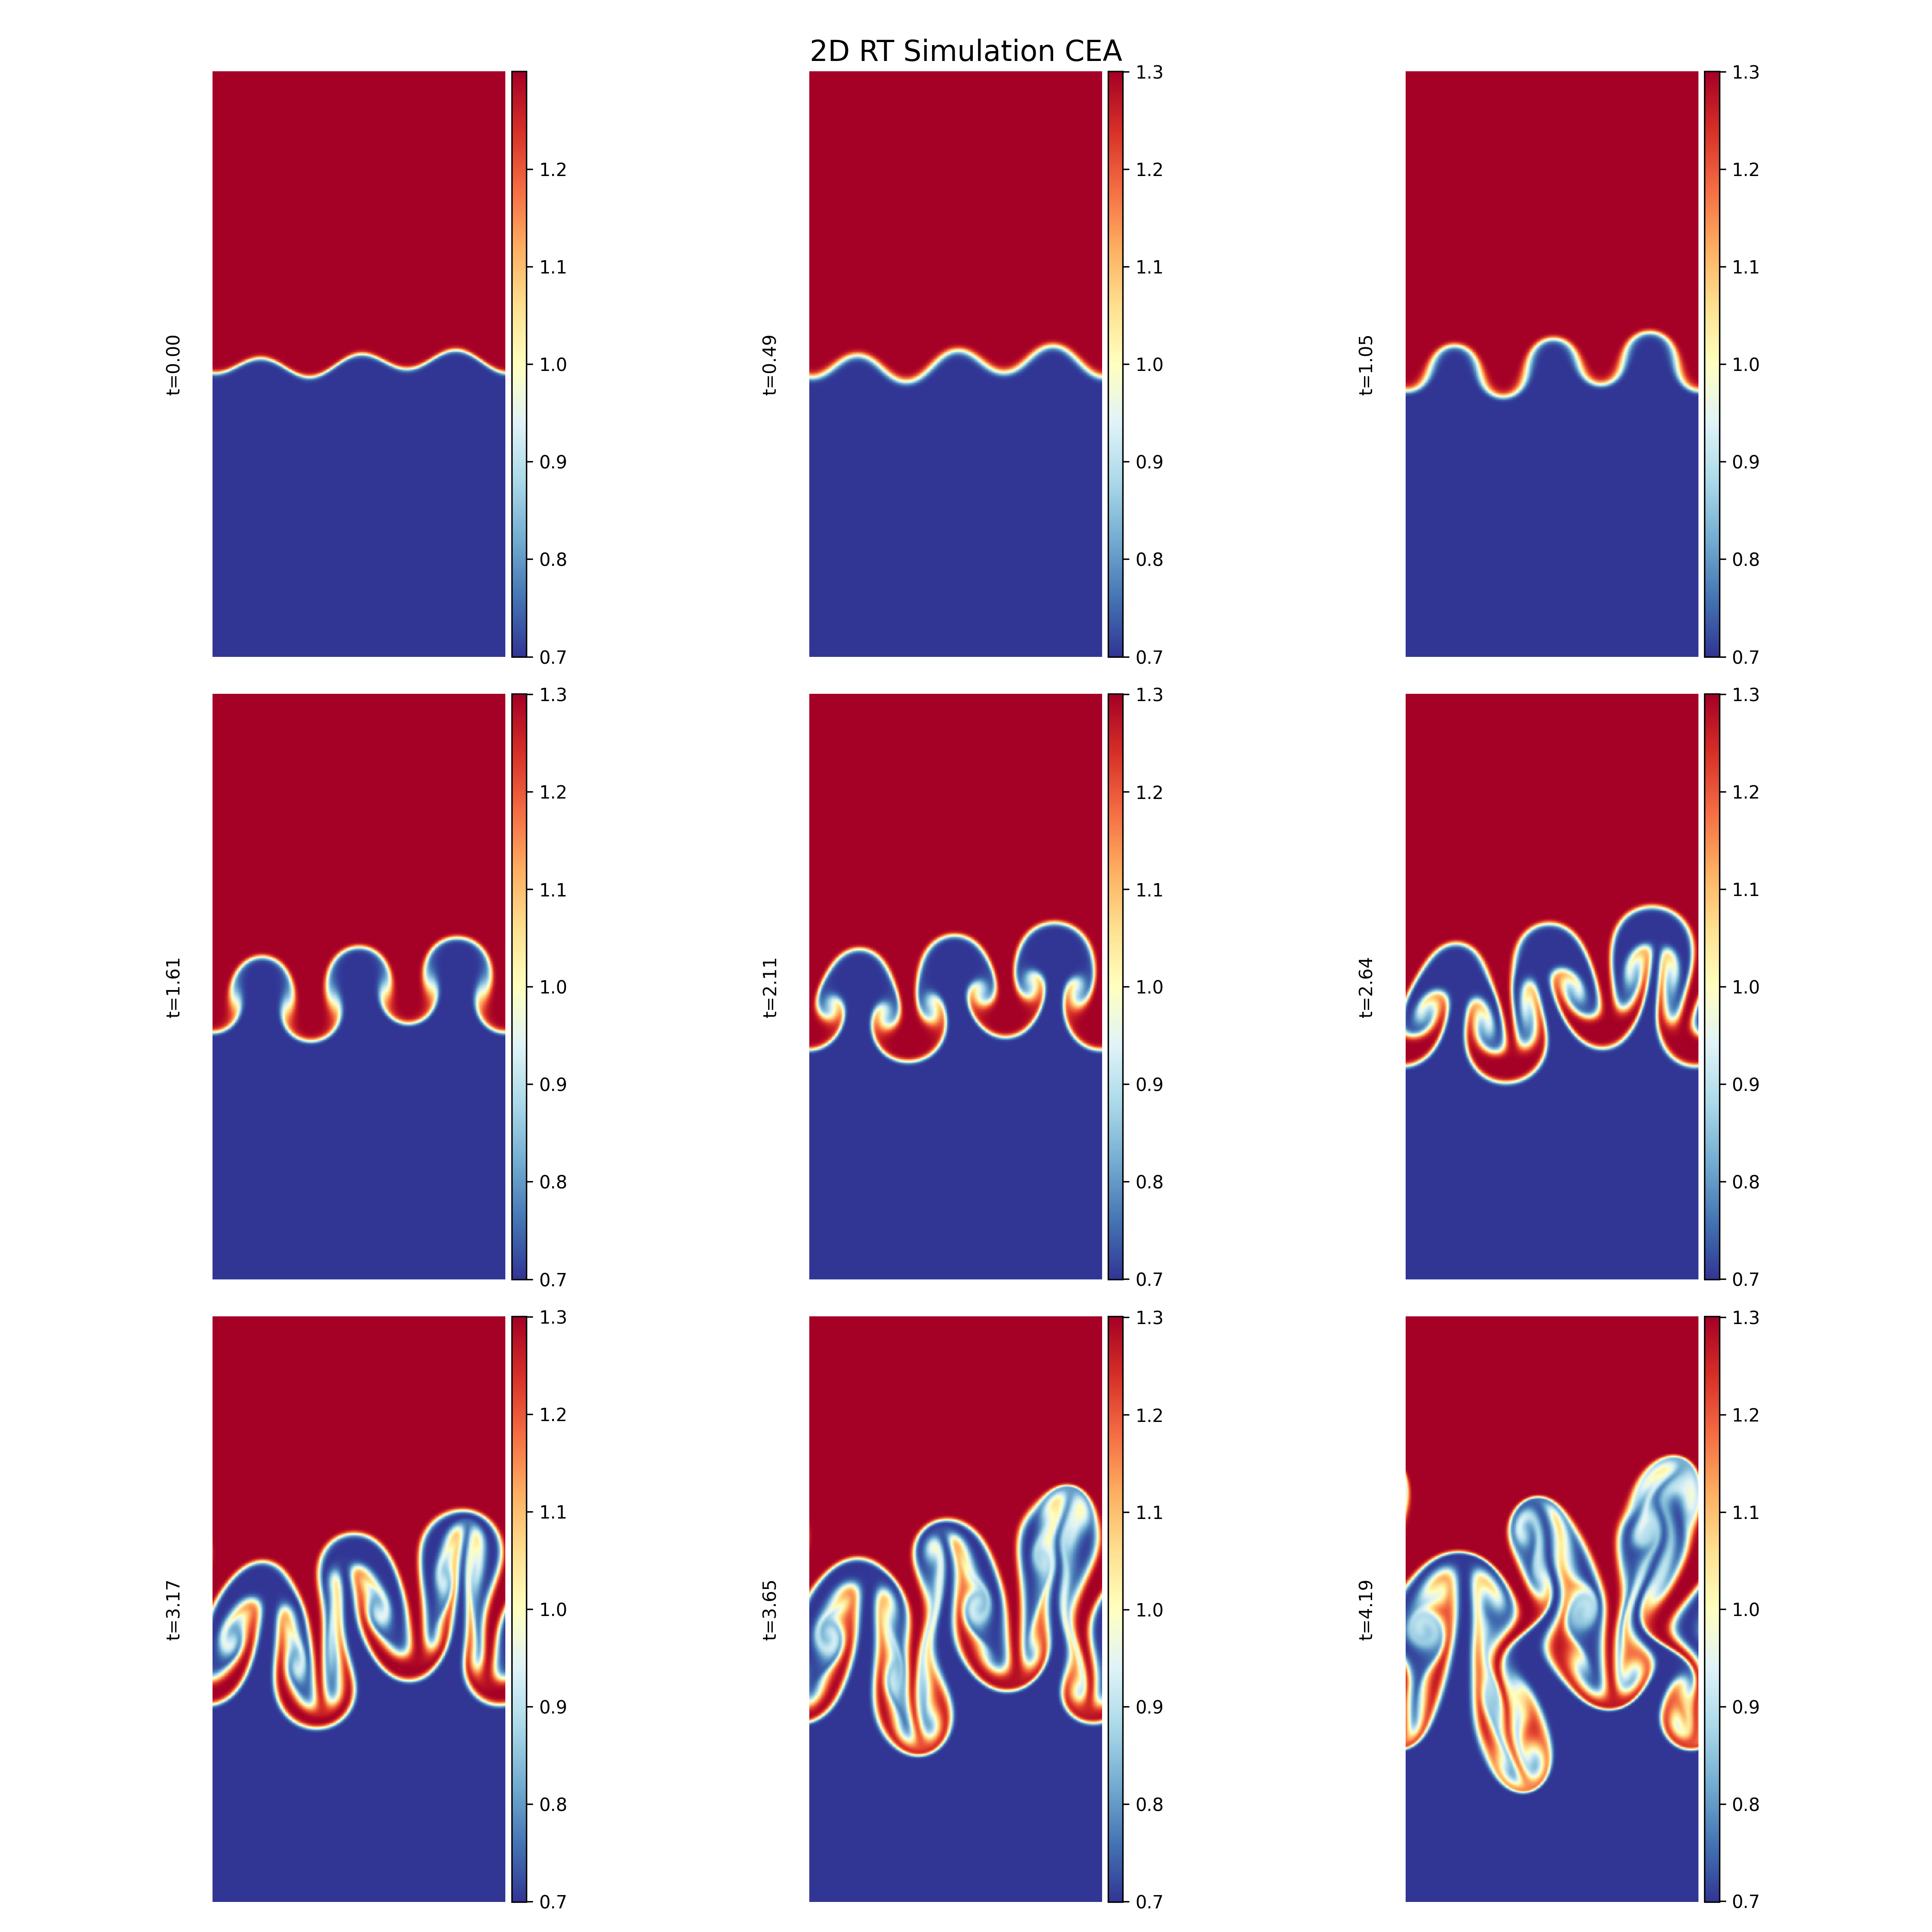
\includegraphics[width=\linewidth,height=0.65\textheight,keepaspectratio]{figures/RTCEA_simulation_2D.png}

      \vspace{0.4ex}
      {\tiny Évolution d'un champ de densité issu d'une simulation directe.}

    \end{column}

    \begin{column}{0.54\textwidth}
      \begin{block}{Approche du projet}
        \small
        Apprendre la distribution des champs 2D pour générer de nouveaux échantillons à coût réduit.

        \vspace{0.4ex}
        {\scriptsize\color{CEAblue}\textbf{Hypothèse :} les ondelettes préservent mieux les structures localisées avec peu de données.}
      \end{block}

      \vspace{0.1ex}
      \centering
      \begin{tikzpicture}[
          node distance=1.7mm,
          box/.style={draw=CEAblue,fill=CEAblue!8,rounded corners=1.5pt,
            align=center,minimum height=6mm,text width=3.4cm,font=\scriptsize},
          arrow/.style={-{Latex[length=1.5mm]},thick,draw=CEAred}
        ]
        \node[box] (dns) {Simulations\\Rayleigh--Taylor};
        \node[box,below=of dns] (repr) {Prétraitement puis\\Fourier / ondelettes};
        \node[box,below=of repr] (ddpm) {Modèle de diffusion\\DDPM\textsuperscript{1}};
        \node[box,below=of ddpm] (eval) {Évaluation visuelle,\\statistique et physique};
        \draw[arrow] (dns) -- (repr);
        \draw[arrow] (repr) -- (ddpm);
        \draw[arrow] (ddpm) -- (eval);
      \end{tikzpicture}

    \end{column}
  \end{columns}
  \begin{textblock*}{0.88\paperwidth}(0.075\paperwidth,0.89\paperheight)
    {\tiny\color{CEAgrey}
    \textsuperscript{1}\textbf{DDPM} : Denoising Diffusion Probabilistic Model.}
  \end{textblock*}
\end{frame}

% ============================================== %

\begin{frame}[plain]
  \frametitle{Pourquoi les ondelettes ?}
  % \framesubtitle{Raconter les structures multi-échelles avec peu de coefficients}
  \vspace{-3ex}

  \begin{columns}[T,onlytextwidth]
    \begin{column}{0.40\textwidth}
      \centering

      \vspace{0.4ex}
      
\includegraphics[width=0.9\linewidth,keepaspectratio]{figures/2DExemple_Reconstruction.png}

      \vspace{0.4ex}
      
\includegraphics[width=0.9\linewidth,keepaspectratio]{figures/2DExemple_Masque.png}

    \end{column}

    \begin{column}{0.56\textwidth}
      % \begin{block}{Structures RT}
      %   \scriptsize
      %   \begin{itemize}
      %     \item Discontinuités : interfaces et fronts de densité.
      %     % \item Grandes structures : bulles et doigts de Rayleigh--Taylor.
      %     % \item Petites structures : filaments et instabilités secondaires.
      %     \item Multi-échelles : les structures sont hiérarchiques et imbriquées.
      %   \end{itemize}
      % \end{block}

      % \vspace{0.5ex}
      \begin{block}{Représentation parcimonieuse}
        \scriptsize
        Les ondelettes gardent les coefficients là où le champ porte l'information.\\
        \vspace{5px}
        {\scriptsize\color{CEAblue}\textbf{Note :} Image d'illustration est de forme volontairement specifique pour visualiser les structures multi-échelles.}
      \end{block}

      \begin{block}{Ondelettes pour la diffusion}
      \end{block}

      \vspace{-2ex}
      \begin{center}
        
\includegraphics[width=\linewidth,height=0.6\textheight,keepaspectratio]{figures/WaveletDiffusion.png}
      \end{center}
      
    \end{column}
  \end{columns}
  \begin{textblock*}{0.35\paperwidth}(0.62\paperwidth,0.925\paperheight)
    {\hfill\usebeamerfont{footline}\color{CEAlightgrey}23/06/2026\hspace{20pt}%
    \textbf{\color{CEAred}\insertframenumber{} / \inserttotalframenumber}}
  \end{textblock*}
\end{frame}

% ============================================== %

\begin{frame}
  \frametitle{Premiers résultats : baseline DDPM}
  \framesubtitle{Des champs plausibles, à valider par des métriques physiques}

  \begin{columns}[T,onlytextwidth]
    \begin{column}{0.30\textwidth}
      \centering
      \textbf{Données de référence}

      \vspace{0.6ex}
      
\includegraphics[width=\linewidth,height=0.55\textheight,keepaspectratio]{figures/original.png}
    \end{column}

    \begin{column}{0.30\textwidth}
      \centering
      \textbf{Champs générés}

      \vspace{0.6ex}
      
\includegraphics[width=\linewidth,height=0.55\textheight,keepaspectratio]{figures/generated.png}
    \end{column}

    \begin{column}{0.36\textwidth}
      \begin{block}{Validation statistique}
        \scriptsize
        \begin{itemize}
          \item PhyFID\textsuperscript{1} : \textbf{0.189} pour les champs générés ;
          \item ordre de grandeur proche du témoin validation/train : \textbf{0.11} ;
          \item bruit et MNIST restent très éloignés : \textbf{18.0} et \textbf{15.3}.
        \end{itemize}
      \end{block}

      \vspace{-1ex}
      \begin{alertblock}{Lecture physique}
        \scriptsize
        Les profils moyens par ligne sont bien reproduits :
        \(d_\mu=\textbf{0.0017}\), \(d_\sigma=\textbf{0.0021}\)
        à comparer à respectivemetn \(>0.07\) et \(>0.02\) pour MNIST/bruit.

        \vspace{0.5ex}
        Le spectre des fluctuations est également bien reproduit :
        \(d_E=\textbf{0.1608}\), à comparer à \(>4\) pour MNIST/bruit.

        \vspace{0.5ex}
        \textbf{Suite :} diffusion en ondelettes et métriques physiquement informées.
      \end{alertblock}
    \end{column}
  \end{columns}
  \begin{textblock*}{0.88\paperwidth}(0.075\paperwidth,0.89\paperheight)
    {\tiny\color{CEAgrey}\textsuperscript{1}\textbf{PhyFID} : FID calculé dans un espace de features appris sur les simulations Rayleigh--Taylor.}
  \end{textblock*}
\end{frame}

\begin{frame}[plain]
  \usebeamertemplate*{last page}
\end{frame}

\end{document}
